\documentclass[12pt]{article}

%------------------------
% Packages
%------------------------
\usepackage{graphicx}
\usepackage{float}

\usepackage[a4paper,margin=1in]{geometry}
\usepackage{caption}
\captionsetup{font=small}
\usepackage{amsmath,amssymb}
\usepackage{amsthm}
\usepackage{graphicx}
\usepackage{hyperref}
\usepackage{physics}
\usepackage{setspace}
\usepackage[
    backend=biber,
    style=numeric,
    sorting=none,
    maxcitenames=2,
    maxbibnames=99,
    giveninits=true
]{biblatex}

\addbibresource{Plasma_Thesis.bib}
\setstretch{1.25}

%------------------------
% Title Page
%------------------------
\begin{document}

\begin{titlepage}
    \centering

    {\Large\bfseries
    Nonlinear Cross-Correlation Analysis of Plasma Turbulence in Magnetically Confined Fusion Devices\\[0.5cm]}

    {\large PHYS 493.6 --- Midterm Report\\[1cm]}

    {\large
    \textbf{Jayneel Parikh}\\
    Department of Physics \& Engineering Physics\\
    University of Saskatchewan\\[0.5cm]
    Under the supervision of \textbf{Dr.\ Chijin Xiao}\\[2cm]}
    {\Large December 2025}


%------------------------
% Abstract
%------------------------
\begin{abstract}
Plasma transport in magnetically confined fusion devices exceeds classical and neoclassical predictions by more than an order of magnitude, largely due to turbulence driven by drift-type instabilities. Conventional linear correlation methods fail to fully characterize turbulent interactions because they assume Gaussian statistics and provide no information about the direction of coupling between fluctuation signals. To overcome these limitations, Ding \textit{et al.} \cite{dingNonlinearRadialCorrelation1997} introduced a nonlinear cross-correlation method based on conditional dispersion in reconstructed phase space. This technique extracts both the strength and direction of coupling between two fluctuating signals. Similarly, van Milligen \textit{et al.} \cite{vanmilligenRadialPropagationHeat2019} introduces a information theoretic approach using transfer entropy.  In this project, the algorithm is implemented and validated using synthetic data generated from coupled Van der Pol oscillators, a system with well-defined and well studied master–slave dynamics.  Preliminary applications to experimental floating-potential signals from the HT7 tokomak demonstrate the method's ability to detect directional propagation of turbulence energy.
\end{abstract}

\end{titlepage}

\newpage

%------------------------
% Objectives
%------------------------

%------------------------
% Introduction
%------------------------

\section{Introduction}

\subsection{Motivation}

Since the earliest tokamak experiments, particle and heat losses have consistently exceeded both
classical and neoclassical predictions. Major devices such as PLT, ASDEX, and TFTR reported
cross-field diffusivities one to two orders of magnitude larger than collisional theory allows, as
reviewed by Carreras \cite{carrerasProgressAnomalousTransport1997}. These results established a
central fact of magnetic-confinement research: transport in toroidal plasmas is dominated not by
collisions, but by turbulence.

Understanding how turbulent structures propagate across radii is therefore essential for explaining
energy confinement. Classical diagnostics typically rely on linear tools such as cross-correlation
and spectral analysis. However, linear correlation assumes Gaussian statistics and coherent
waveform propagation; it therefore cannot reliably capture deformation under shear, nor can it
identify directional coupling between spatially separated signals. These limitations become more
severe near confinement transitions, where turbulence reorganizes on millisecond timescales.

To overcome these issues, Ding~\textit{et al.} introduced a nonlinear cross-correlation method for
the STOR--M tokamak \cite{dingNonlinearRadialCorrelation1997}. By reconstructing local
dynamics via delay-coordinate embedding \cite{takensDetectingStrangeAttractors1981,
gutmanTakensEmbeddingTheorem2015} and measuring conditional dispersion between neighborhoods
in two signals, the method extracts both (i) a nonlinear correlation strength $g_{xy}$ and
(ii) a directional asymmetry
\[
S_{xy} = \frac{g_{xy}-g_{yx}}{g_{xy}+g_{yx}},
\]
which reveals whether turbulent energy preferentially propagates inward or outward. This approach
successfully identified direction reversals during L--H transitions in STOR--M, and subsequent
applications in TJ-II reproduced similar behavior under electrode biasing
\cite{bsharatConditionalCrosscorrelationAnalysis2024}.

Complementary nonlinear techniques reinforce the same physical picture. Transfer entropy (TE),
applied extensively in toroidal plasmas \cite{vanmilligenCausalityDetectionTurbulence2013,
vanmilligenRadialPropagationHeat2019}, measures information flow between fluctuations and has
revealed nonlocal ``jumping'' heat propagation and fast/slow transport channels. While TE and
Ding's method differ in formulation, both aim to quantify directional, nonlinear coupling in
turbulent systems. This conceptual overlap provides motivation to better understand what aspects
of causality or propagation are captured by conditional dispersion.

The present work implements and validates the nonlinear cross-correlation method of
Ding~\textit{et al.} and applies it to floating-potential fluctuations from fusion plasmas.
The goal is to extract nonlinear correlation lengths, determine propagation direction, and provide
a diagnostic framework for turbulence-driven transport beyond what linear statistics can reveal.

\subsection{Transport Regimes in Plasmas}

\subsubsection*{Classical Transport}

Classical diffusion arises from Coulomb collisions. In an unmagnetized plasma, particles undergo a
random walk with diffusion coefficient
\[
D \sim v_{\mathrm{th}}^{2}\tau = \frac{\lambda_m^{2}}{\tau},
\]
where $v_{\mathrm{th}}$ is the thermal speed, $\lambda_m$ the mean free path, and
$\tau = \nu^{-1}$ the collision time for collision frequency $\nu$
\cite{chenIntroductionPlasmaPhysics2016}. In a magnetic field $\mathbf{B}$, charged particles gyrate
with Larmor radius
\[
\rho_L = \frac{v_\perp}{\omega_c} = \frac{m v_\perp}{q B},
\]
where $v_\perp$ is the perpendicular velocity, $q$ the charge, $m$ the mass, and
$\omega_c = qB/m$ the cyclotron frequency. Collisions randomize the gyro-phase, giving a
perpendicular diffusion coefficient
\[
D_{\perp} = \nu \rho_L^2 = \frac{K T \nu}{m\omega_c^2},
\]
with temperature $T$ and Boltzmann constant $K$
\cite[§5.5]{chenIntroductionPlasmaPhysics2016}.
Classical transport is small because $\rho_L$ is small in strong magnetic fields.

\subsubsection*{Neoclassical Transport}

Toroidal geometry introduces magnetic curvature and trapped-particle orbits (“banana” trajectories),
which increase the effective radial step size. This yields neoclassical diffusion
$D_{\mathrm{neo}} > D_{\perp}$, but still typically far below experimental values
\cite{carrerasProgressAnomalousTransport1997}.

\subsubsection*{Anomalous Transport}

Measured transport $D_{\mathrm{exp}}$ often exceeds $D_{\mathrm{neo}}$ by one to two orders of magnitude.
This discrepancy is attributed to turbulence: fluctuations in density $n$, electrostatic potential
$\phi$, and temperature $T$ drive cross-field $\mathbf{E}\times\mathbf{B}$ flows, forming eddies that
enhance radial mixing. These fluctuations are intermittent, non-Gaussian, and strongly nonlinear.
Linear diagnostics underestimate correlation lengths and cannot determine causal propagation
direction. Nonlinear approaches, including conditional-dispersion analysis
\cite{dingNonlinearRadialCorrelation1997} and transfer-entropy methods
\cite{vanmilligenCausalityDetectionTurbulence2013,vanmilligenRadialPropagationHeat2019},
offer a path toward resolving these properties and clarifying the dynamics responsible for
turbulent transport.

\section{Experimental Setup}

This work analyzes two types of data: (i) synthetic time series generated from coupled
Van der Pol oscillators, used to validate the nonlinear cross-correlation algorithm, and
(ii) floating-potential fluctuations measured in fusion plasmas using Langmuir probes.

\subsection{Synthetic Data: Coupled Van der Pol Oscillators}

Following Ding~\textit{et al.}~\cite{dingNonlinearRadialCorrelation1997}, we first validate the nonlinear conditional correlation (NLCC) algorithm using a pair of coupled nonlinear oscillators whose direction of interaction is known \emph{a priori}. Both Ding and van Milligen use the same general Van-der-Pol form,
\[
    \ddot{x} = \left(a_1 - (x + b y)^2\right)\dot{x} - (x + b y), \qquad
    \ddot{y} = \left(a_2 - (y + a x)^2\right)\dot{y} - (y + a x),
\]
but they operate in \emph{different parameter regimes}, producing qualitatively different dynamics.
The parameters $a,b$ determine the direction and strength of coupling: when $|a| > |b|$, oscillator~$x$ drives 
oscillator~$y$, and vice versa.

We numerically integrate both systems using a fixed time step $\Delta t = 0.01\,\mathrm{s}$ (matching the 
sampling resolution used in van Milligen~(2014)).  
Each resulting time series is normalized window-by-window to reproduce the behaviour of the legacy NLCC 
implementation.

Ding's parameter choice ($a_1 = a_2 = 1$, $a = 0.5$, $b = -2.5$) lies in a strongly nonlinear regime, producing 
a distorted, multi-loop quasi-periodic attractor with noticeable amplitude modulation.  
In contrast, the parameters used by van Milligen et al.\ (2014) 
($a_1 = 1$, $a_2 = 1.1$, with only unidirectional coupling $x_2 \rightarrow x_1$) generate a 
thin quasi-periodic torus resembling a clean limit cycle, consistent with two slightly detuned oscillators.  
These distinctions provide a clear comparison point when applying NLCC: Ding’s system stresses the algorithm 
with strong nonlinear interactions, while the van Milligen system provides a more regular and interpretable benchmark.

Figures~\ref{fig:ding_ts}--\ref{fig:vm_phase} show the corresponding time series and phase-space trajectories.

% --------------------------------------------------------------
% Ding time series
% --------------------------------------------------------------
\begin{figure}[H]
    \centering
    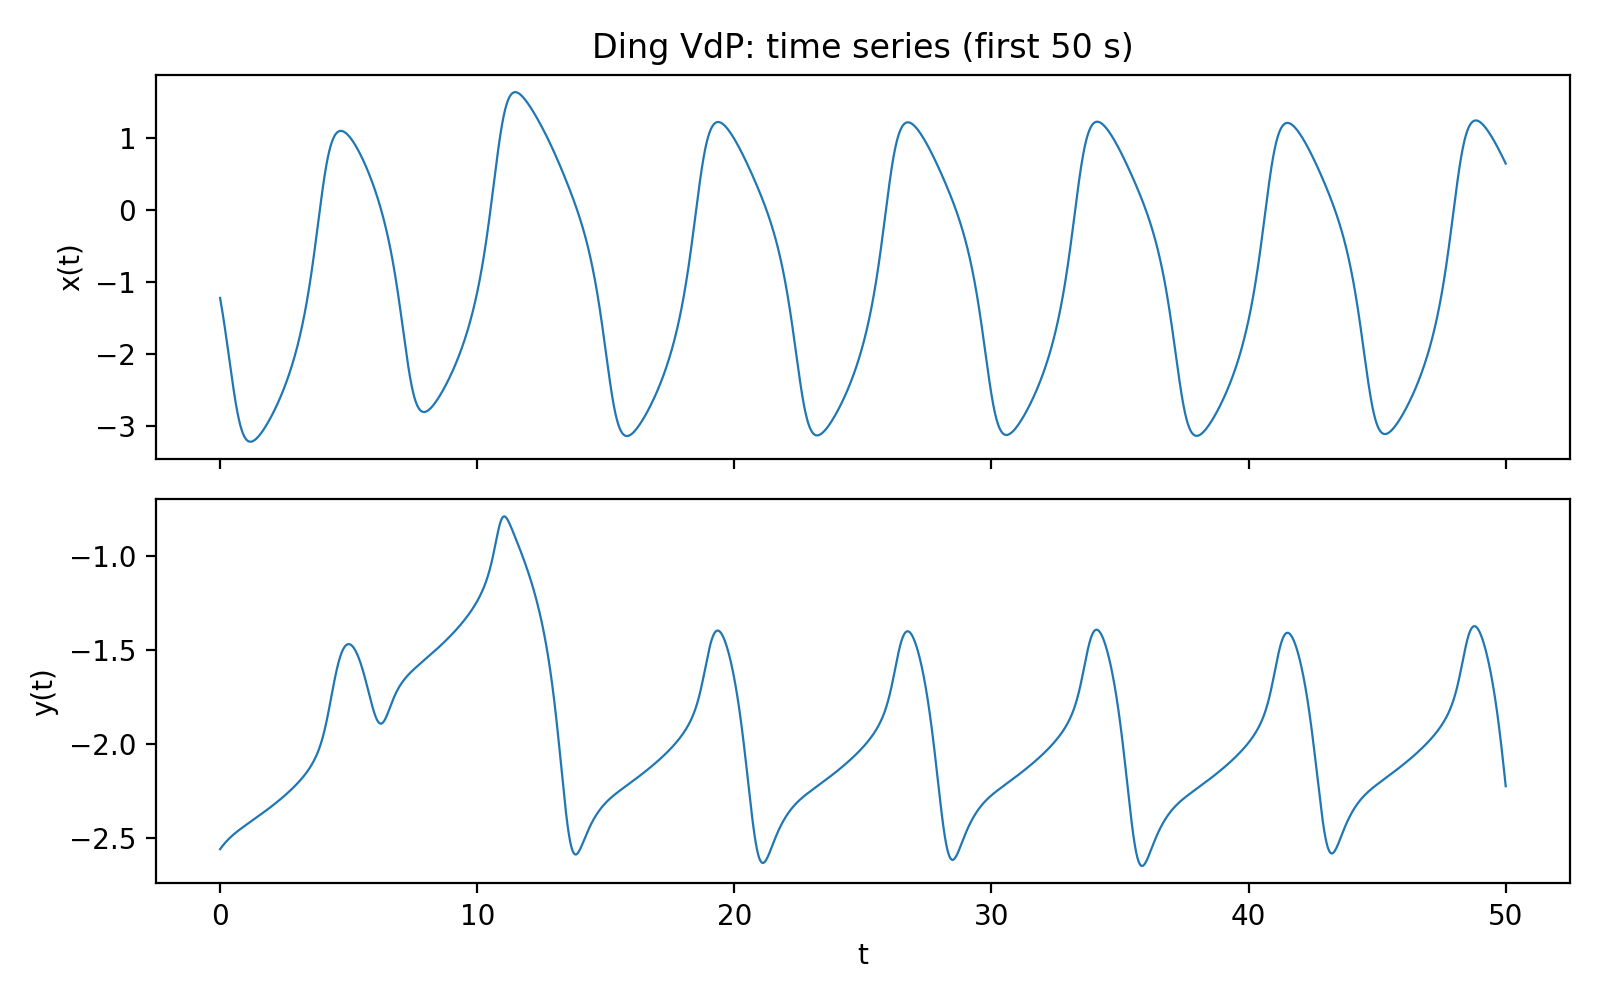
\includegraphics[scale=0.35]{ding_timeseries.png}
    \caption{Time series of the Ding coupled oscillator system 
    ($a_1=a_2=1$, $a=2.5$, $b=-0.5$).  
    The pronounced cycle-to-cycle modulation reflects quasi-periodic dynamics with strong nonlinear coupling.}
    \label{fig:ding_ts}
\end{figure}

% --------------------------------------------------------------
% Ding phase space
% --------------------------------------------------------------
\begin{figure}[H]
    \centering
    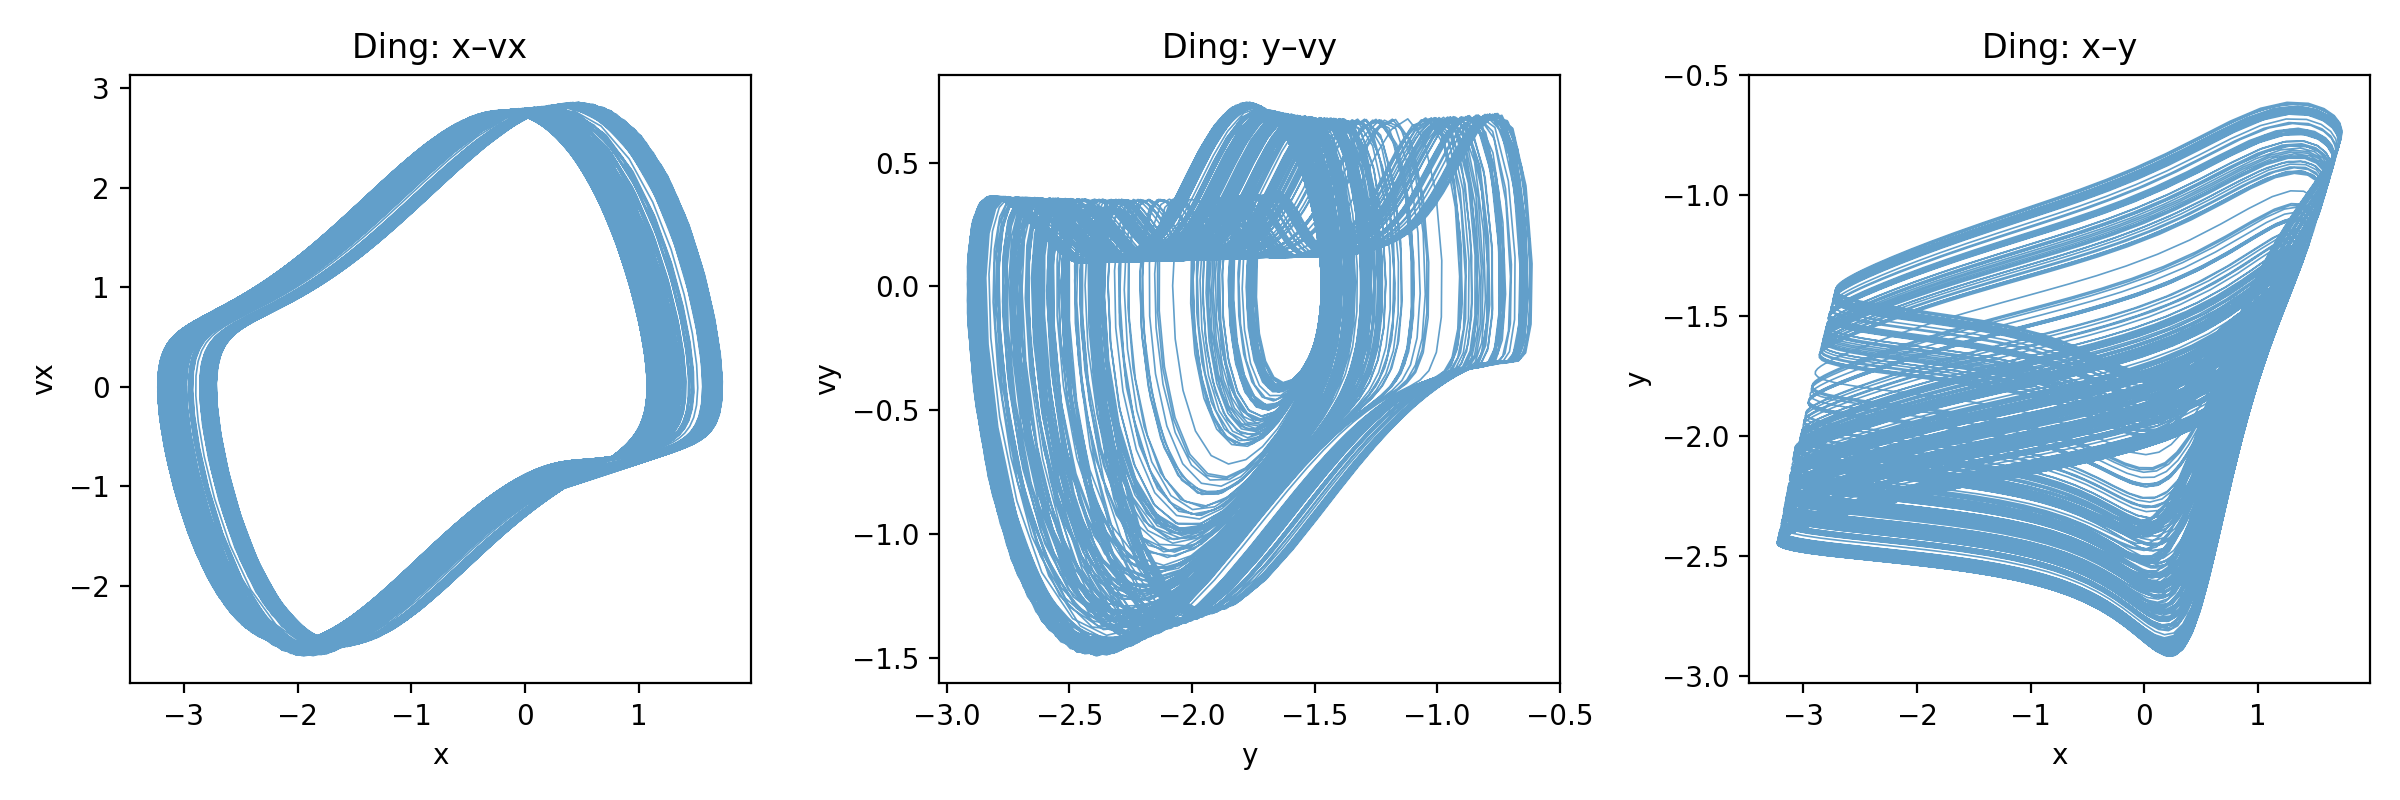
\includegraphics[scale=0.35]{ding_phase_space.png}
    \caption{Phase-space projections of the Ding system.  
    The thickened, multi-loop structure indicates a quasi-periodic attractor with amplitude modulation, 
    in contrast to the thin closed orbit of a simple Van der Pol limit cycle.}
    \label{fig:ding_phase}
\end{figure}

% --------------------------------------------------------------
% VM time series
% --------------------------------------------------------------
\begin{figure}[H]
    \centering
    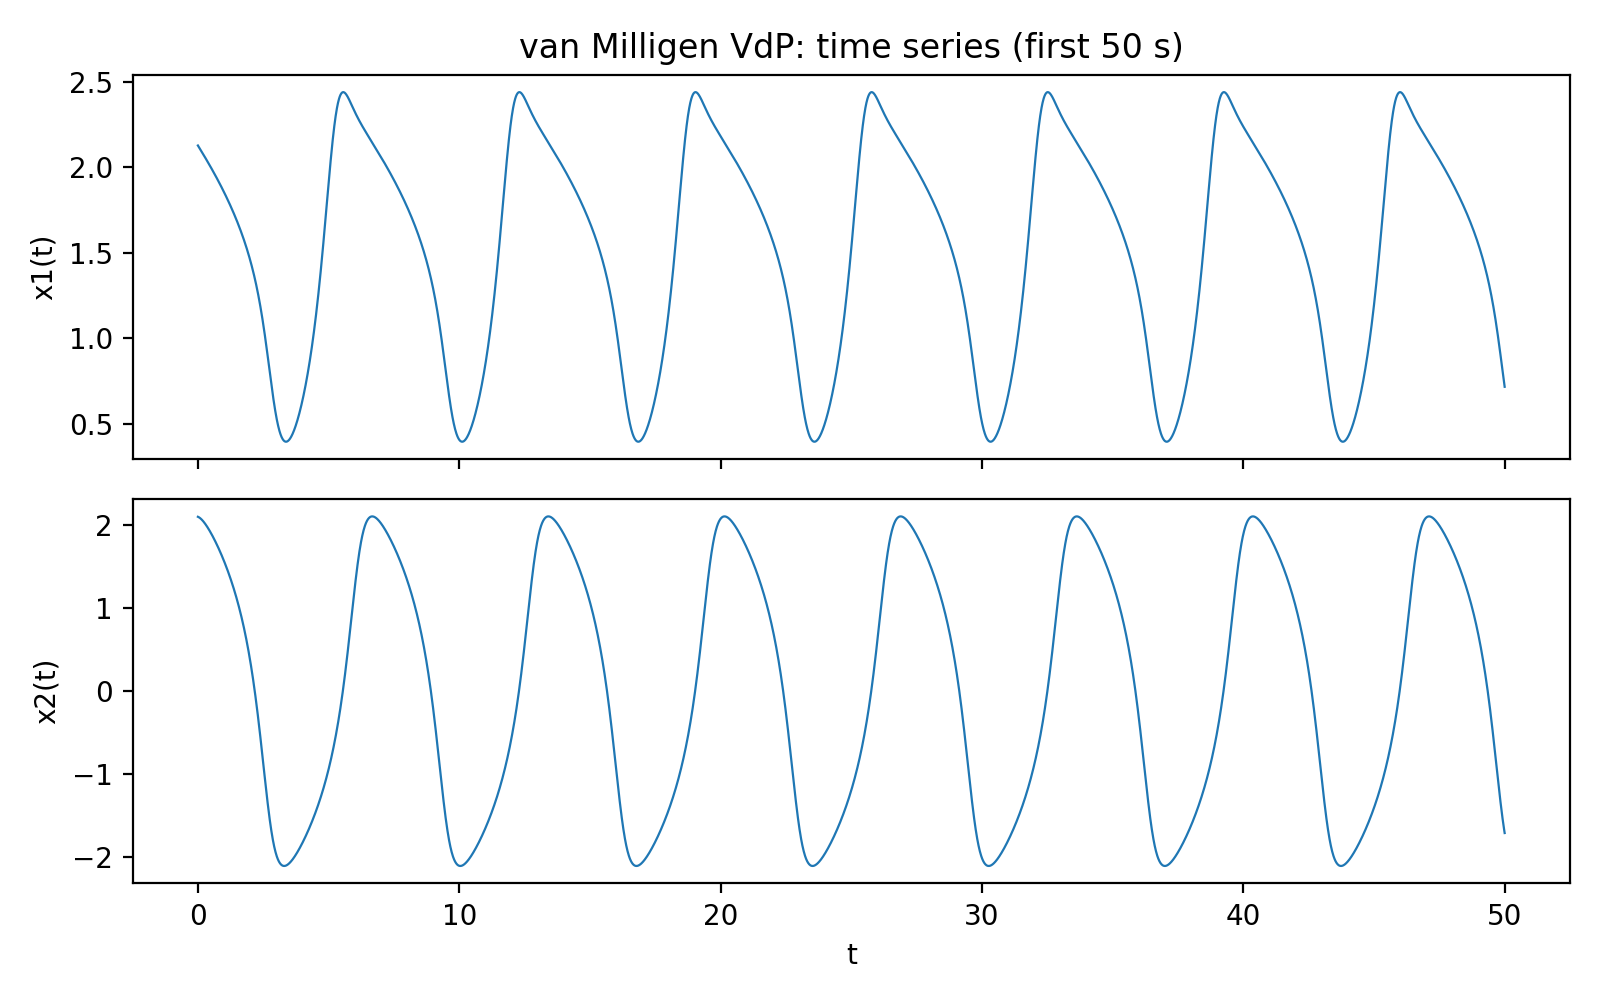
\includegraphics[scale=0.35]{vm_timeseries.png}
    \caption{Time series of the van Milligen (2014) oscillator pair 
    ($a_1 = 1$, $a_2 = 1.1$, unidirectional coupling $x_2 \rightarrow x_1$).  
    The dynamics are nearly periodic, with only slight modulation arising from detuning.}
    \label{fig:vm_ts}
\end{figure}

% --------------------------------------------------------------
% VM phase space
% --------------------------------------------------------------
\begin{figure}[H]
    \centering
    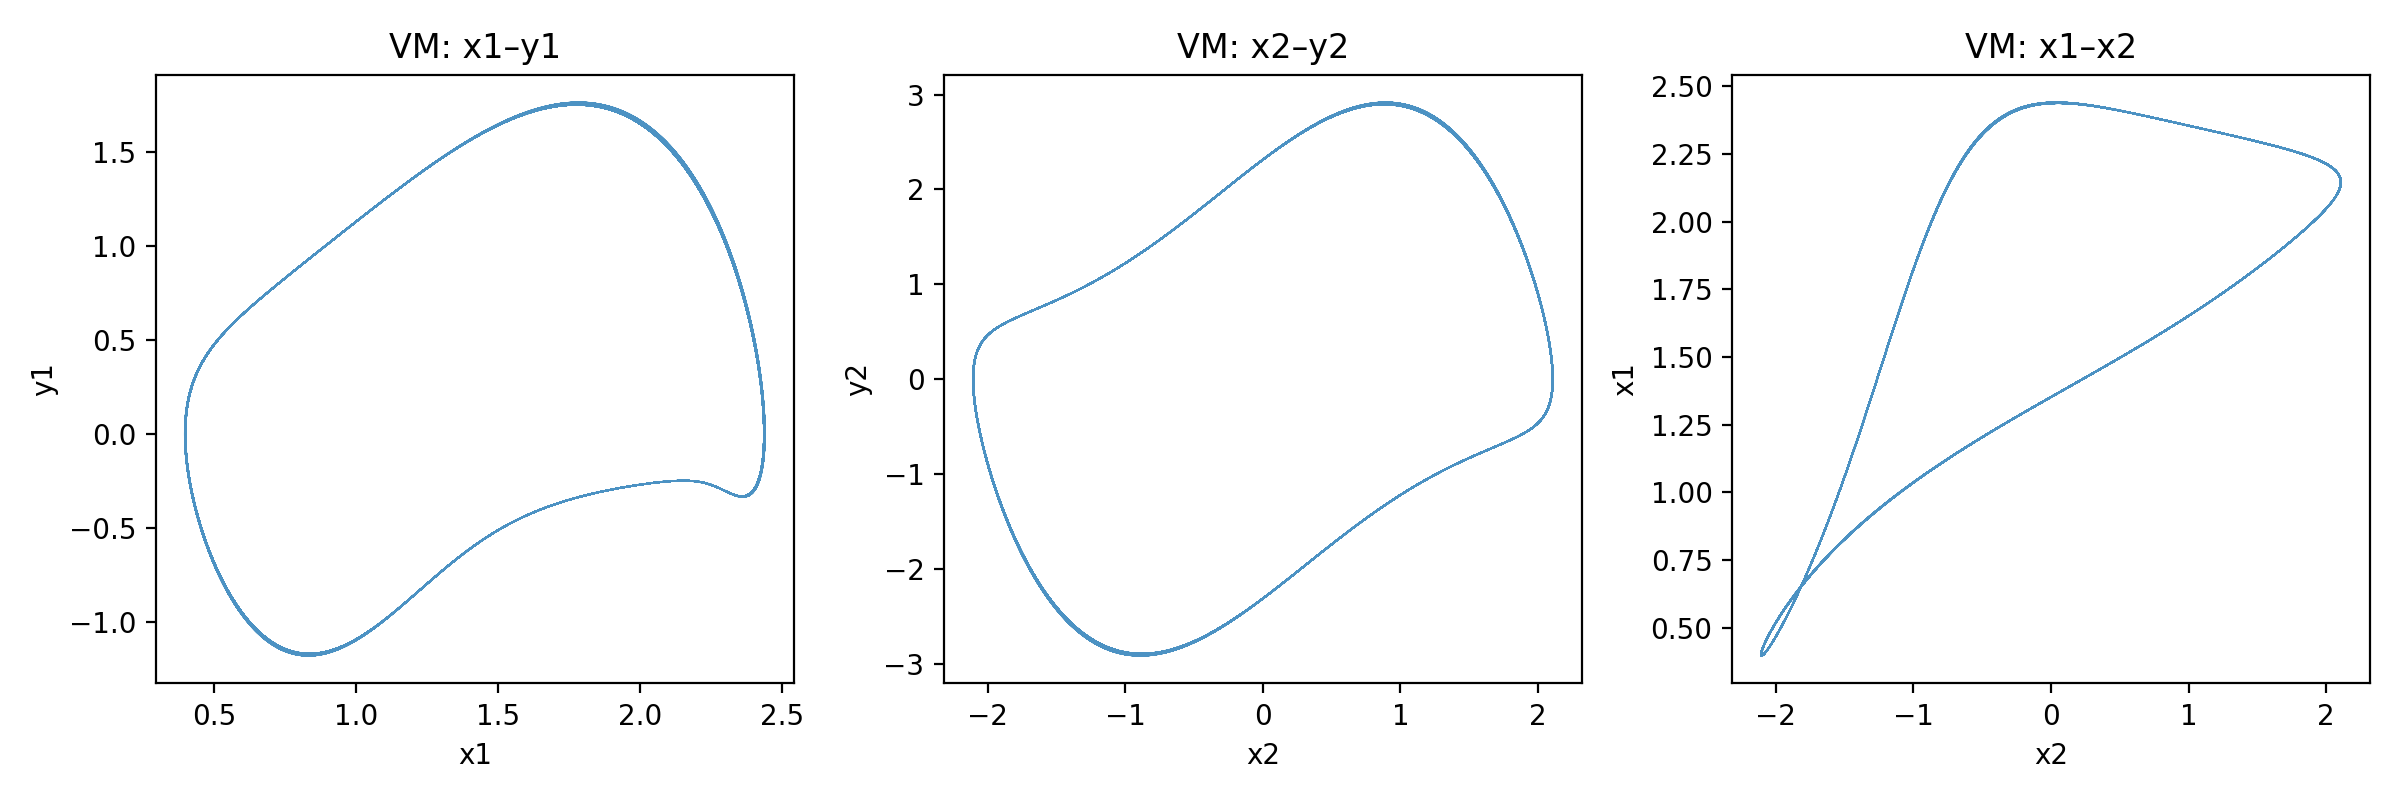
\includegraphics[scale=0.35]{vm_phase_space.png}
    \caption{Phase-space projections of the van Milligen system.  
    Each oscillator approaches a thin quasi-periodic torus resembling a limit cycle, and the $(x_1,x_2)$ 
    projection clearly shows unidirectional driving from oscillator~2 to oscillator~1.}
    \label{fig:vm_phase}
\end{figure}
\subsection{Experimental Data: Floating-Potential Fluctuations}

The primary experimental data used in this study consist of floating-potential signals
$\tilde{V}_f(t)$ measured by radially separated Langmuir probe tips in a magnetically confined
plasma. Depending on the device, the probes are inserted near the edge region where turbulent
fluctuations are strongest.

In the STOR--M tokamak, Ding~\textit{et al.}~\cite{dingNonlinearRadialCorrelation1997}
used two tips separated by a radial distance $\Delta r$ to detect outward and inward propagation
across the L--H transition. More recent work on the TJ-II stellarator has used multi-pin rake
probes with millimetre-scale separations, allowing directional coupling to be measured across a
range of radial positions \cite{bsharatConditionalCrosscorrelationAnalysis2024}.

In the present study, we analyse floating-potential recordings from the HT-7 tokamak, provided in
the legacy \texttt{A.dat}/\texttt{B.dat} format. Each probe provides a scalar signal,
\[
    x(t) = \tilde{V}_f(r_1,t), \qquad
    y(t) = \tilde{V}_f(r_2,t),
\]
	sampled at frequency $f_s=1/\Delta t$.  Following the conventions of the original NLCC code, the signals are detrended and normalized within each analysis window to avoid biasing the conditional-dispersion measure. 
	
	Figure~\ref{fig:ht7_overview_ts} shows the first $50\,\mathrm{ms}$ of the discharge. During this interval the plasma evolves from a low-amplitude state into a regime of strong intermittent bursts, followed by fully developed broadband turbulence. This “global view’’ is provided to emphasize that HT-7 fluctuations are neither periodic nor quasi-periodic, in stark contrast to the synthetic Van der Pol systems studied earlier. However, the NLCC algorithm requires a locally stationary segment. Therefore, the actual analysis is performed on short windows (e.g.\ $100$--$105\,\mathrm{ms}$), where the fluctuations have settled into a statistically steady turbulent state.  Figure~\ref{fig:ht7_window_ts} shows $x(t)$ and $y(t)$ over such a window.  Unlike the synthetic systems, the fluctuations have no clearly defined phase or amplitude structure, and correlation must be inferred from the underlying statistics rather than from coherent cycles.

To visualize the underlying dynamics in a coordinate-free way, we construct a two-dimensional delay embedding of the form $(x(t),\,x(t+\tau))$ using the same delay $\tau$ as in the NLCC analysis.  Figure~\ref{fig:ht7_embed} shows the resulting embedding for a representative HT-7 signal.  Instead of lying on a thin one-dimensional curve (as in a periodic oscillator) or a smooth torus (as in the quasi-periodic Van der Pol case), the points fill a thick, irregular region.  This is typical of broadband turbulent fluctuations with rapidly decorrelating amplitudes and phases.  Such features motivate the use of nonlinear directional metrics like NLCC rather than traditional linear cross-correlation.

% --------------------------------------------------------------
% Combined time series figure
% --------------------------------------------------------------
\begin{figure}[H]
    \centering

    % --- Left: full 50 ms overview ---
    \begin{minipage}{0.42\textwidth}
        \centering
        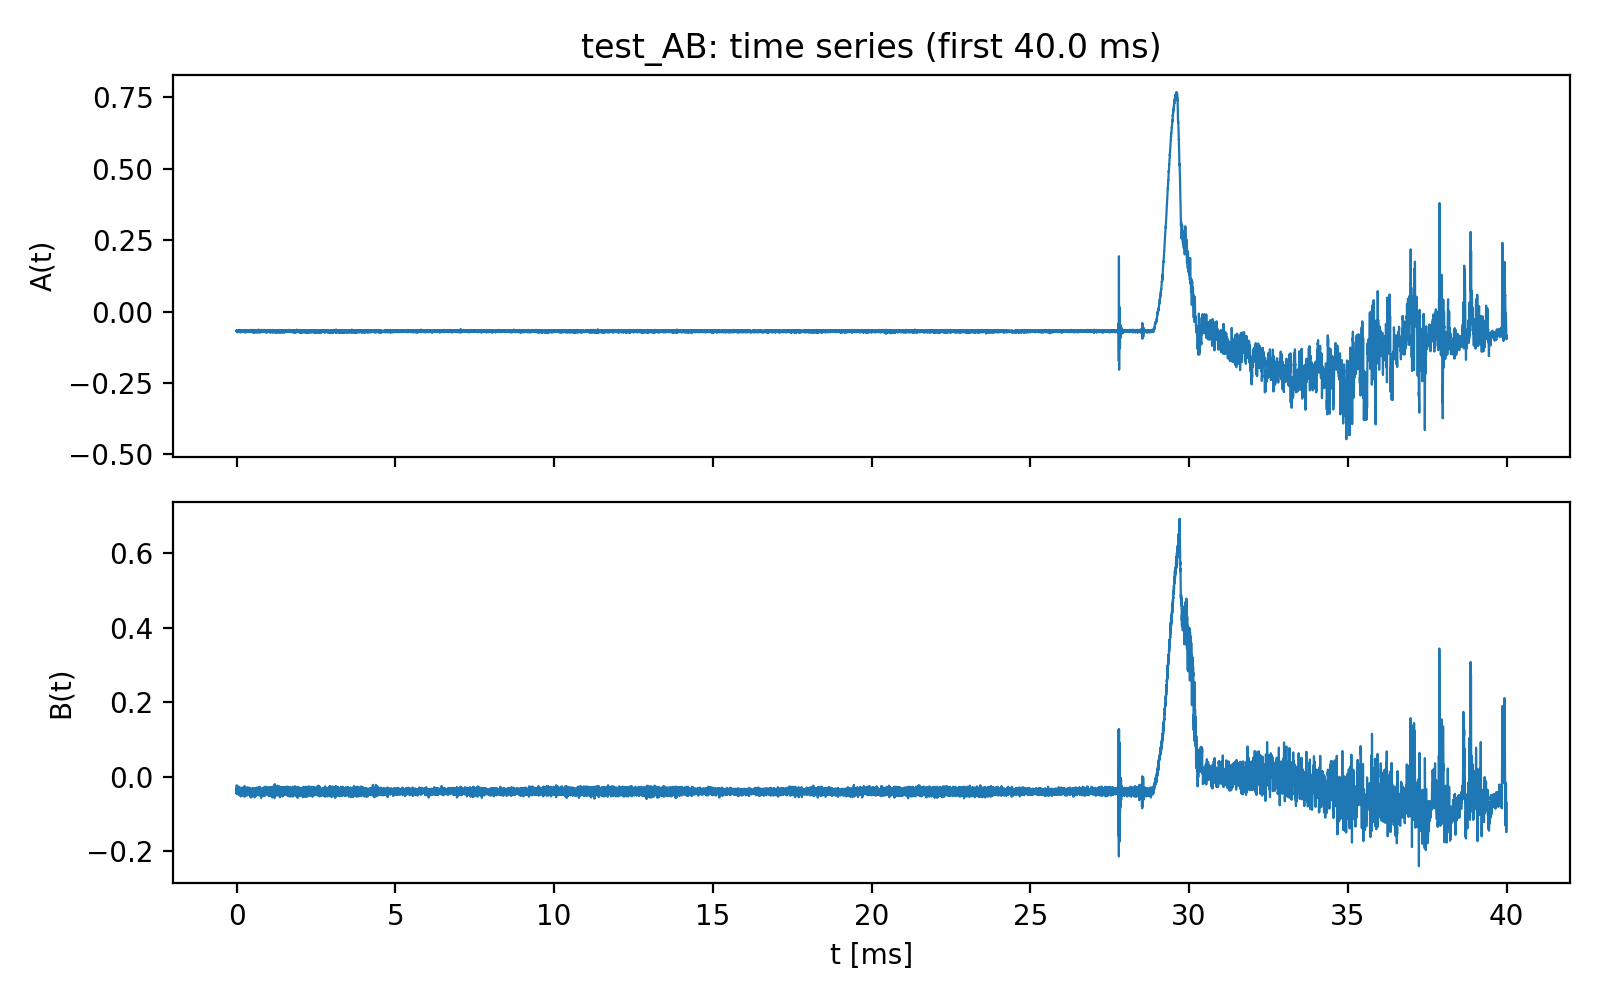
\includegraphics[width=\textwidth]{test_AB_timeseries.png}
        \caption{Overview time series ($0$--$50$ ms).}
    \end{minipage}
    \hfill
    % --- Right: NLCC window ---
    \begin{minipage}{0.42\textwidth}
        \centering
        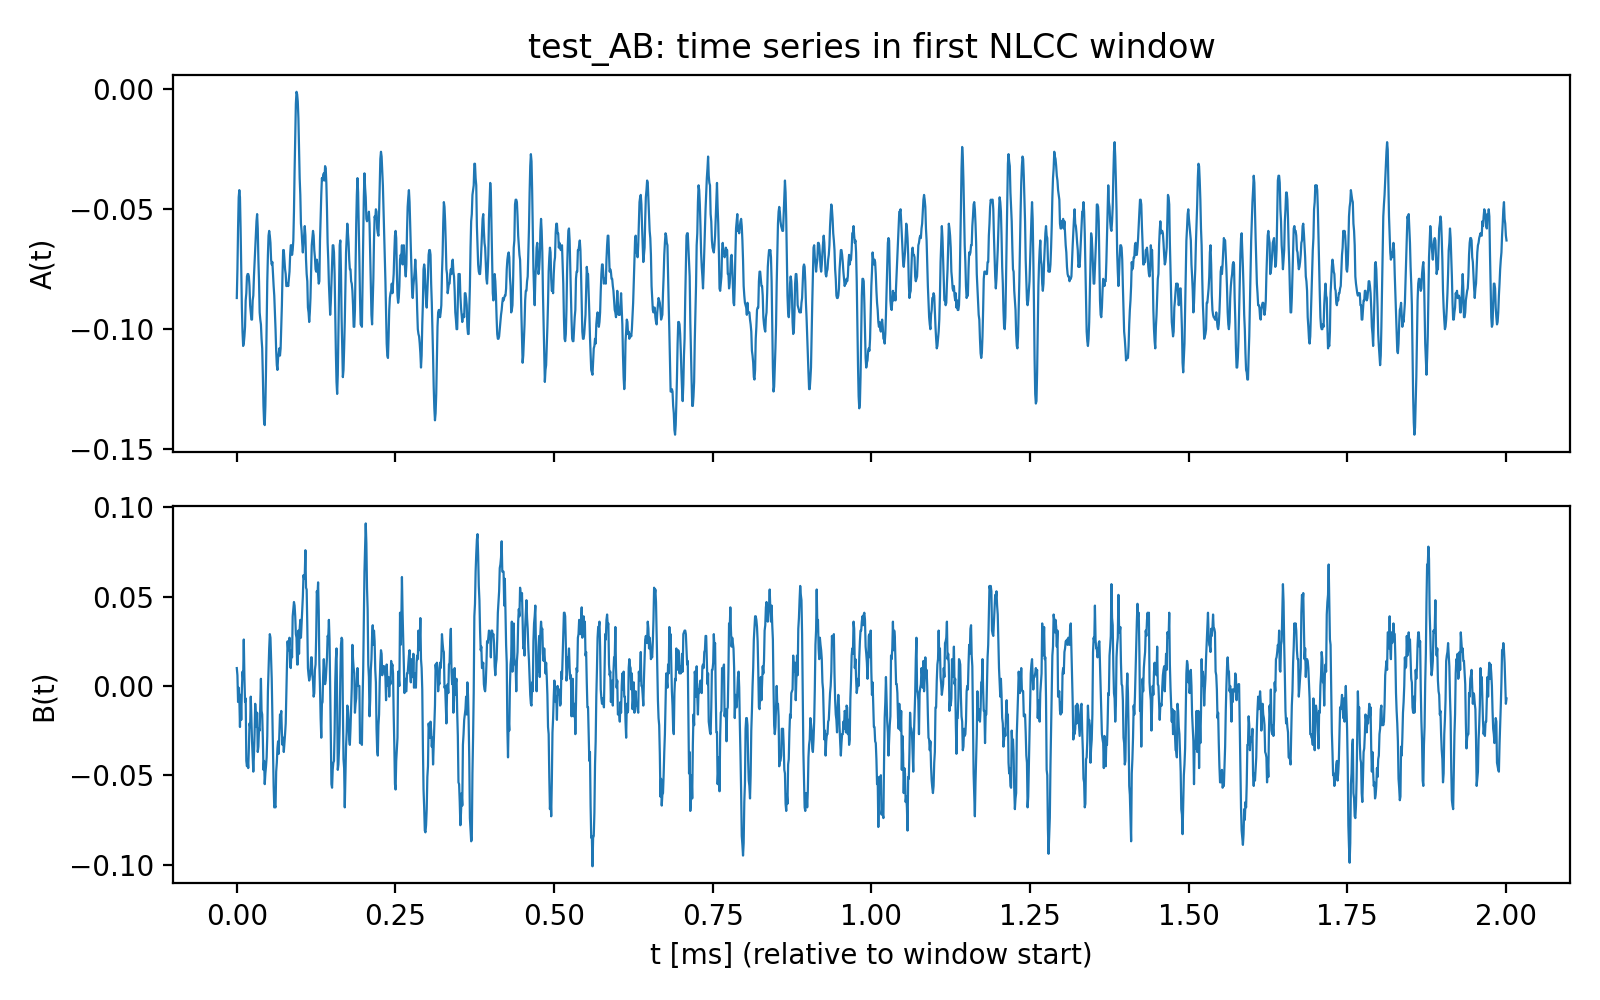
\includegraphics[width=\textwidth]{test_AB_timeseries_window.png}
        \caption{NLCC analysis window ($100$--$105$ ms).}
    \end{minipage}
\end{figure}% --------------------------------------------------------------
% Delay embedding (D=2)
% --------------------------------------------------------------
\begin{figure}[H]
    \centering
    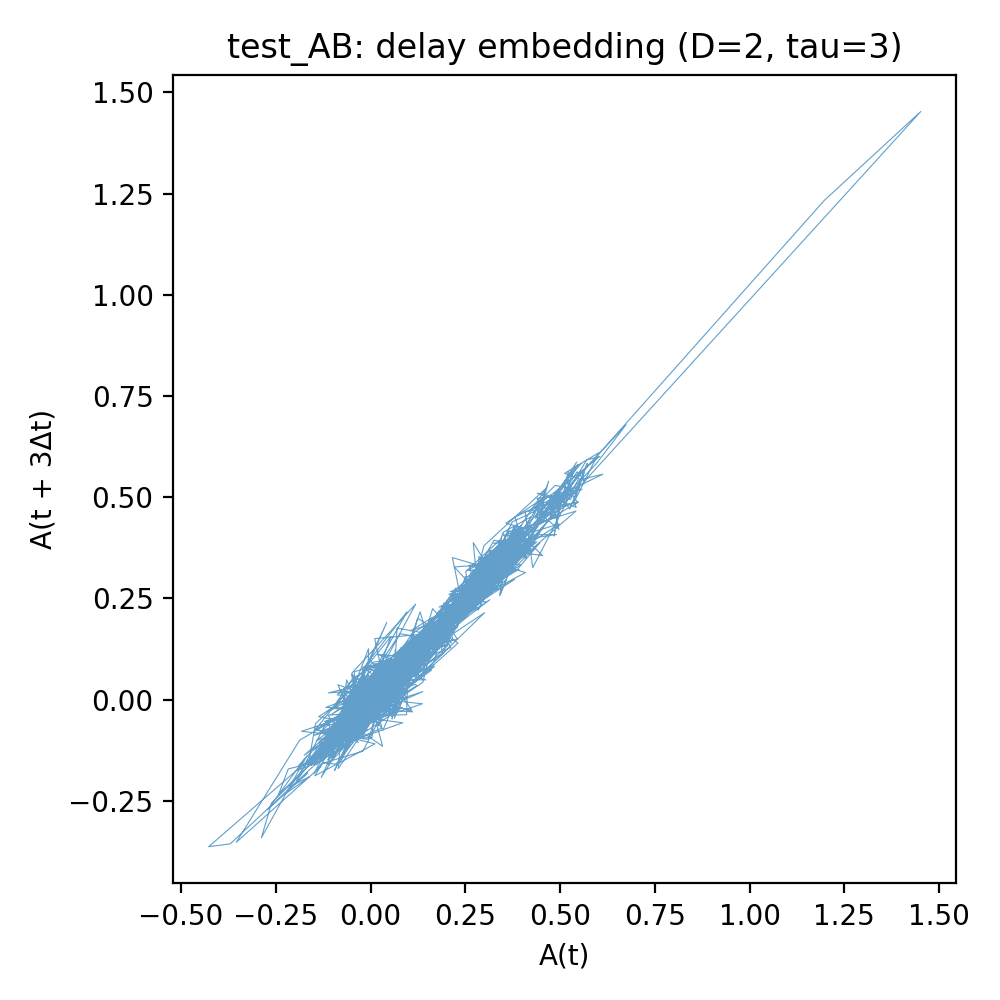
\includegraphics[scale = 0.42]{test_AB_embed_D2.png}
    \caption{Two-dimensional delay embedding $(x(t), x(t+\tau))$ of the HT-7 floating-potential
    signal using the same delay $\tau$ as in the NLCC analysis.}
     \label{fig:ht7_embed}
\end{figure}

\subsection{Windowing, Embedding, and Preprocessing}

The nonlinear correlation method operates on fixed-length windows of size $N$ samples. For each
time window:
\begin{itemize}
    \item The signals are normalized to zero mean and unit variance.
    \item A delay time $m$ is chosen near the first minimum of the autocorrelation function.
    \item Embedding dimension $M$ is varied from $1$ to $9$ to test saturation of the conditional
          dispersion curve, following Ding’s prescription.
    \item All computations use overlapping windows, stepped by $\Delta t_{\mathrm{win}}$,
          enabling time-resolved estimation of propagation direction.
\end{itemize}

These parameters match the procedures used in both STOR--M and TJ-II analyses
\cite{dingNonlinearRadialCorrelation1997,bsharatConditionalCrosscorrelationAnalysis2024} and are chosen to ensure comparability with established results in the literature. The resulting embedded vectors $\{X_i^{(M)}\}$ and $\{Y_i^{(M)}\}$ form the input to the conditional-dispersion algorithm described in the next section.

\section{ Nonlinear Correlation: Theory}

\subsection{Why linear correlation fails}

The linear cross-correlation between two signals \(x(t)\) and \(y(t)\),
\[
C_{xy}(\tau)
=
\frac{\langle x(t)\,y(t+\tau)\rangle}
{\sqrt{\langle x^{2}\rangle\,\langle y^{2}\rangle}},
\]
where $\langle\,\cdot\,\rangle$ denote a time average over the analysis window, measures phase coherence but cannot detect nonlinear dependence.
As emphasized by Ding \textit{et al.}\ \cite{dingNonlinearRadialCorrelation1997}, this creates three problems for turbulent plasmas:  
(i) \(C_{xy}=0\) does not imply independence unless the joint statistics are Gaussian, and edge fluctuations are strongly non-Gaussian;  
(ii) shear and waveform distortion reduce linear correlation lengths even when the underlying dynamics remain related;  
(iii) long averaging times are required for convergence, making the method insensitive to rapid changes and unable to indicate directionality.  
These limitations motivate a nonlinear approach based on reconstructed dynamics.

\subsection{ Phase–space reconstruction and conditional dispersion}

Given a scalar signal \(x(t)\), Ding’s method reconstructs the local dynamics using delay embedding.  
For a chosen delay \(m\) (in samples) and embedding dimension \(M\), the delay vector
\[
X_i^{(M)}
=
\frac{1}{\sqrt{M}}\,(x_i,\,x_{i+m},\,\dots,\,x_{i+(M-1)m})
\]
represents the system state at sample \(i\).  
The identical construction applied to \(y(t)\) yields delay vectors \(Y_i^{(M)}\).  
If the signals are dynamically related, proximity in the \(X\)-space tends to imply proximity in the \(Y\)-space; if they are independent, distances in \(Y^{(M)}\) contain no information about distances in \(X^{(M)}\).

To quantify this relationship, Ding \textit{et al.}\ define the conditional dispersion
\[
\sigma_{xy}^{(M)}(\varepsilon)
=
\sqrt{
\frac{
\sum_{i\neq j}
\lVert Y_i^{(M)}-Y_j^{(M)}\rVert^{2}
\,H\!\bigl(\varepsilon-\lVert X_i^{(M)}-X_j^{(M)}\rVert\bigr)
}{
\sum_{i\neq j}
H\!\bigl(\varepsilon-\lVert X_i^{(M)}-X_j^{(M)}\rVert\bigr)
}},
\]
where \(\varepsilon\) is a scale parameter, \(\lVert \cdot \rVert\) is the Euclidean norm in \(\mathbb{R}^M\),  
and \(H\) is the Heaviside function.  
The quantity \(\sigma_{xy}^{(M)}(\varepsilon)\) measures the rms spread of the \(Y\)-vectors associated with \(X\)-vectors lying within an \(\varepsilon\)-ball.

Let \(\sigma_{\max}^{(M)}\) be the maximum over the scanned range of \(\varepsilon\), and let \(\varepsilon_{90}^{(M)}\) satisfy \(\sigma_{xy}^{(M)}(\varepsilon_{90}^{(M)})=0.9\,\sigma_{\max}^{(M)}\).  
If \(\varepsilon_{\max}=\max_{i,j}\lVert X_i^{(M)}-X_j^{(M)}\rVert\), the nonlinear correlation coefficient from \(x\) to \(y\) is
\[
g_{xy}^{(M)}=\frac{\varepsilon_{90}^{(M)}}{\varepsilon_{\max}}.
\]
For practical purposes \(g_{xy}^{(M)}\) saturates for \(M\simeq 7\!-\!9\), at which point we write \(g_{xy}\).  
Exchanging the roles of \(x\) and \(y\) yields \(g_{yx}\).  
Self–correlation coefficients \(g_{xx}\) and \(g_{yy}\) are obtained by applying the same procedure to a single signal; the normalized measure \(G_{xy}=g_{xy}/\sqrt{g_{xx}g_{yy}}\) compensates for differing fluctuation amplitudes.

Because the construction is directional, \(g_{xy}\neq g_{yx}\).  
Using the corrected sign convention (the original expression in \cite{dingNonlinearRadialCorrelation1997} contains a misprint), the directional asymmetry is
\[
S_{xy}
=
\frac{g_{xy}-g_{yx}}{g_{xy}+g_{yx}},
\]
so that \(S_{xy}>0\) indicates a stronger influence from \(x\) to \(y\), and \(S_{xy}<0\) indicates the reverse.

\subsection{Algorithm validation}

Ding \textit{et al.}\ validated this method using the coupled Van der Pol oscillators introduced earlier in Section~2, whose coupling direction is known from the parameters \(a\) and \(b\).  
The nonlinear coefficients correctly reproduce the expected master–slave relationship: when \(|a|>|b|\), one finds \(g_{xy}>g_{yx}\); when \(|a|<|b|\), the inequality reverses; and symmetric coupling gives \(g_{xy}\approx g_{yx}\).  
The method is robust under moderate noise and applicable to experimental datasets with noise levels of a few percent.

In this work, we repeat the validation in both the strongly nonlinear regime used by Ding and the near–limit–cycle regime studied by van Milligen, and we then apply the same algorithm to floating–potential fluctuations from HT-7.


\section{Results}

The Python implementation of the nonlinear conditional correlation (NLCC)
algorithm was applied to three data sets:
(i) floating–potential fluctuations from the HT--7 tokamak,
(ii) synthetic time series from a pair of coupled Van der Pol oscillators
in the strongly nonlinear (Ding) regime, and
(iii) synthetic time series from a near–limit–cycle (van Milligen) regime.
In all cases the embedding and normalisation procedures follow
Section~3.3, with $M=9$ used for the quoted coefficients.
Directional coupling is inferred from the conditional–dispersion curves
$\sigma_{XY}(\varepsilon)$ and $\sigma_{YX}(\varepsilon)$ and from the
nonlinear correlation coefficients $G_{XY},G_{YX}$ extracted at
$\sigma = 0.9$.

\subsection{HT--7 floating–potential data}

For the HT--7 discharge, the probe pair $(A,B)$ samples floating–potential
fluctuations at two nearby radii in the turbulent edge.
A quasi–stationary window in the broadband phase ($100$--$105\,\mathrm{ms}$)
was selected for NLCC analysis, consistent with the preprocessing in
Section~2.2.

Figure~\ref{fig:ht7_sigma_combined} shows the normalised conditional
dispersion curves for both orderings $(X=A,Y=B)$ and $(X=B,Y=A)$ and for
embedding dimensions $M=5,7,9,11$.  In each ordering the two families
$\sigma_{XY}(\varepsilon)$ and $\sigma_{YX}(\varepsilon)$ are smooth,
monotone in $\varepsilon$, and converge towards unity at large scales,
indicating that the windowed signals are well normalised.  At small
$\varepsilon$ the separation between $\sigma_{XY}$ and $\sigma_{YX}$ is
weak, and reversing the probe roles simply interchanges two very similar
curve sets.

The corresponding nonlinear correlation coefficients at $\sigma=0.9$ and
$M=9$ are $G_{AB} \approx 0.268$ and $G_{BA} \approx 0.262$, with an
asymmetry parameter $S_{AB}\approx -0.013$
(Table~\ref{tab:nlcc_summary}).  Thus, the HT--7 edge signals exhibit
only \emph{small} nonlinear correlation between the two radii and a
similarly small directional asymmetry: NLCC does not reveal a strong,
persistent preference for information flow from $A$ to $B$ or from $B$
to $A$ in this particular turbulent window.  This is consistent with the
broad, irregular delay embedding in Fig.~\ref{fig:ht7_embed}, where many
overlapping turbulent structures contribute to the measured fluctuations.

\subsection{Synthetic Van der Pol oscillators}

To test the directional response of the algorithm on systems with a
known coupling structure, we analysed synthetic data from the coupled
Van der Pol oscillators introduced in Section~2.1:
\[
  \ddot x = \bigl(a_1 - (x + b y)^2\bigr)\dot x - (x + b y),\qquad
  \ddot y = \bigl(a_2 - (y + a x)^2\bigr)\dot y - (y + a x).
\]
The parameters $(a_1,a_2,a,b)$ control self–excitation and cross–coupling,
and the phase–space geometry is illustrated in
Figs.~\ref{fig:ding_ts}--\ref{fig:vm_phase}.  Here we focus on the NLCC
outputs.

\subsubsection*{Ding parameter regime}

In the Ding–style case we use $a_1=a_2=1$, $a=2.5$, $b=-0.5$, which
places the system in a strongly nonlinear regime with a distorted,
multi–loop attractor and cycle–to–cycle amplitude modulation
(Figs.~\ref{fig:ding_ts} and~\ref{fig:ding_phase}).  Because $|b|>|a|$,
the $y$–oscillator enters more strongly into the effective restoring
force and damping of $x$, so one expects a net influence $y\to x$.

The dispersion curves computed from the synthetic time series
(Fig.~\ref{fig:vdp_sigma_combined}, left panel) show a clear but
\emph{moderate} separation between $\sigma_{XY}$ and $\sigma_{YX}$ at
small $\varepsilon$.  At $\sigma=0.9$ and $M=9$ the nonlinear
coefficients are $G_{XY}\approx 0.131$ and $G_{YX}\approx 0.203$, so the
direction consistent with $y$ driving $x$ carries the larger nonlinear
correlation.  The corresponding asymmetry has magnitude
$|S_{XY}|\approx 0.21$ (Table~\ref{tab:nlcc_summary}), indicating a
meaningful directional preference, in line with the anisotropic
coupling in the equations.

\subsubsection*{van Milligen parameter regime}

In the van Milligen–style regime we use slightly detuned self–excitation
($a_1=1$, $a_2=1.1$) with a unidirectional coupling term chosen so that
one oscillator effectively drives the other while both remain close to a
quasi–periodic limit cycle (Figs.~\ref{fig:vm_ts} and~\ref{fig:vm_phase}).
The dynamics are far more regular than in the Ding regime: the phase
relation between the oscillators is tight and the trajectories lie on
thin tori in phase space.

The NLCC curves for this case are shown in
Fig.~\ref{fig:vdp_sigma_combined} (right panel).  Both directions now
exhibit very high nonlinear correlation, with
$G_{XY}\approx 0.843$ and $G_{YX}\approx 0.973$ at $\sigma=0.9$,
reflecting the almost deterministic mapping between the two time series.
The asymmetry $|S_{XY}|\approx 0.07$ is smaller than in the Ding case
but still nonzero: the ordering consistent with the imposed drive
direction reaches the reference level at slightly smaller $\varepsilon$
and remains below the reverse dispersion curve over a broad range of
scales.  In this near–limit–cycle regime NLCC therefore detects both a
strong mutual correlation and a modest directional bias.

\subsection{Comparison}

The numerical results are summarised in Table~\ref{tab:nlcc_summary}.
The HT--7 signals show small nonlinear correlation and only a very weak
directional asymmetry; the Ding system shows lower overall correlation
but the largest relative asymmetry $|S_{XY}|$, consistent with strongly
nonlinear, anisotropic coupling; and the van Milligen system shows very
strong mutual correlation with an intermediate asymmetry.  Across these
three regimes the Python implementation behaves in a physically
reasonable way: it reproduces the expected hierarchy of directional
strength implied by the Van der Pol equations, while indicating that the
experimental HT--7 window is nearly symmetric with respect to the two
probe radii.

\begin{table}[H]
  \centering
  \caption{Summary of NLCC coefficients at $\sigma=0.9$ and embedding
  dimension $M=9$ for experimental HT--7 data and synthetic Van der Pol
  tests.  Here $G_{XY}$ and $G_{YX}$ are the nonlinear correlation
  coefficients in the two directions and $S_{XY}$ measures their
  asymmetry.}
  \label{tab:nlcc_summary}
  \begin{tabular}{lccc}
    \hline
    Data set & $G_{XY}$ & $G_{YX}$ & $S_{XY}$ \\
    \hline
    HT--7, $X=A$, $Y=B$            & 0.268 & 0.262 & $-0.013$ \\
    HT--7, $X=B$, $Y=A$            & 0.262 & 0.268 &  $0.013$ \\
    VdP (Ding parameters)          & 0.131 & 0.203 &  $0.214$ \\
    VdP (VM parameters)            & 0.843 & 0.973 &  $0.072$ \\
    \hline
  \end{tabular}
\end{table}

\section{Conclusion and Future Directions}

This work implemented, validated, and applied the nonlinear conditional correlation (NLCC) method to both synthetic and experimental plasma–turbulence data.  Synthetic tests using coupled Van der Pol oscillators demonstrated that the Python implementation recovers the expected ordering of directional influence across distinct dynamical regimes, from weak but clearly anisotropic coupling (Ding parameters) to strong, nearly deterministic correlations with modest asymmetry (van Milligen regime).  Applied to HT--7 edge fluctuations, NLCC extracted only small nonlinear correlation between adjacent probe radii and no strong directional bias within the analysed window, consistent with the broadband, rapidly decorrelating nature of the underlying turbulence.  These results establish that NLCC behaves predictably across controlled benchmarks and remains stable when applied to experimental data.  Future work will extend the analysis to data sets from other tokomaks. We will perform a comparison with transport transitions, transfer-entropy diagnostics, and other nonlinear measures to better understand causality, propagation, and the structure of plasma turbulence.


\begin{figure}[H]
  \centering

  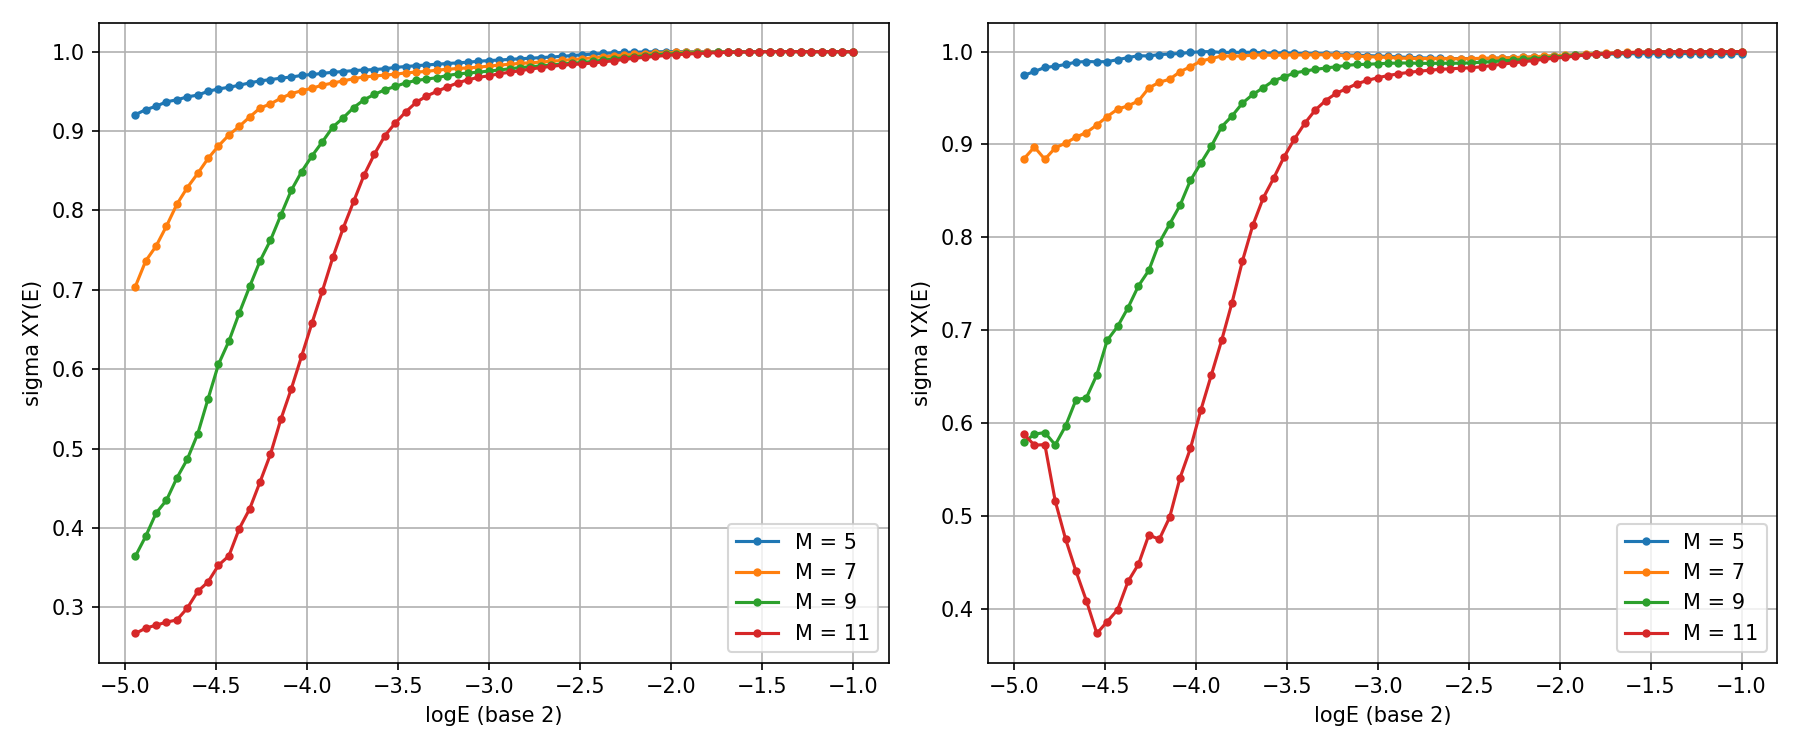
\includegraphics[scale=0.3]{test_AB_figure.png}\hspace{1em}
  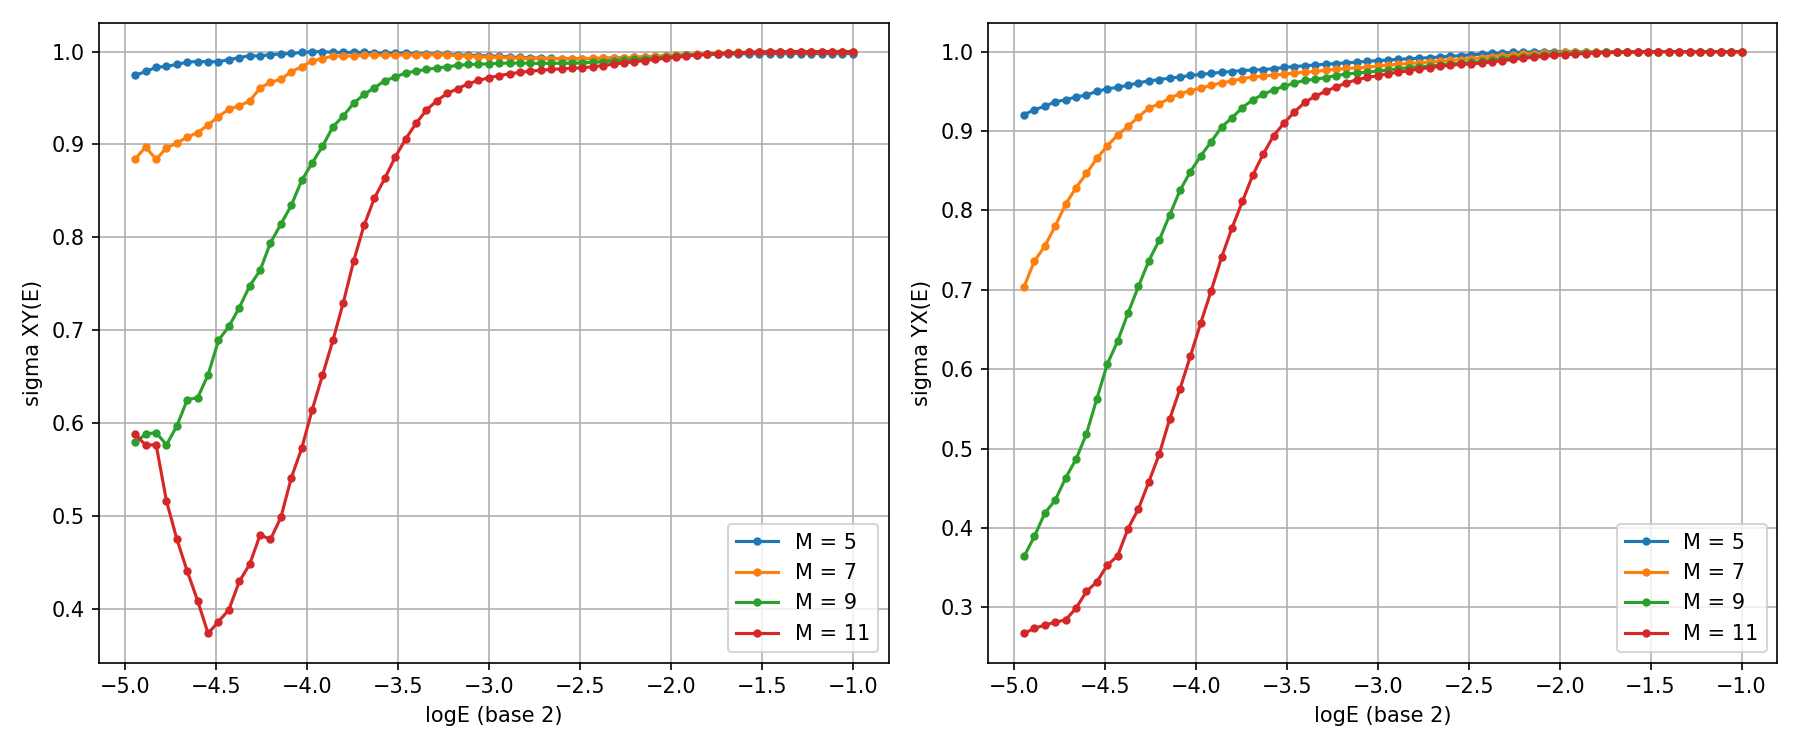
\includegraphics[scale=0.3]{test_BA_figure.png}
  \caption{
    Normalised conditional dispersion curves $\sigma_{XY}(\varepsilon)$ and
    $\sigma_{YX}(\varepsilon)$ for the HT--7 probe pair $(A,B)$ in both
    directions.  Left: $(X=A,Y=B)$; right: $(X=B,Y=A)$.
    The curves are nearly invariant under interchange of the probe roles,
    consistent with the very small directional asymmetry reported in
    Table~\ref{tab:nlcc_summary}.
  }
  \label{fig:ht7_sigma_combined}
\end{figure}

\begin{figure}[H]
  \centering
  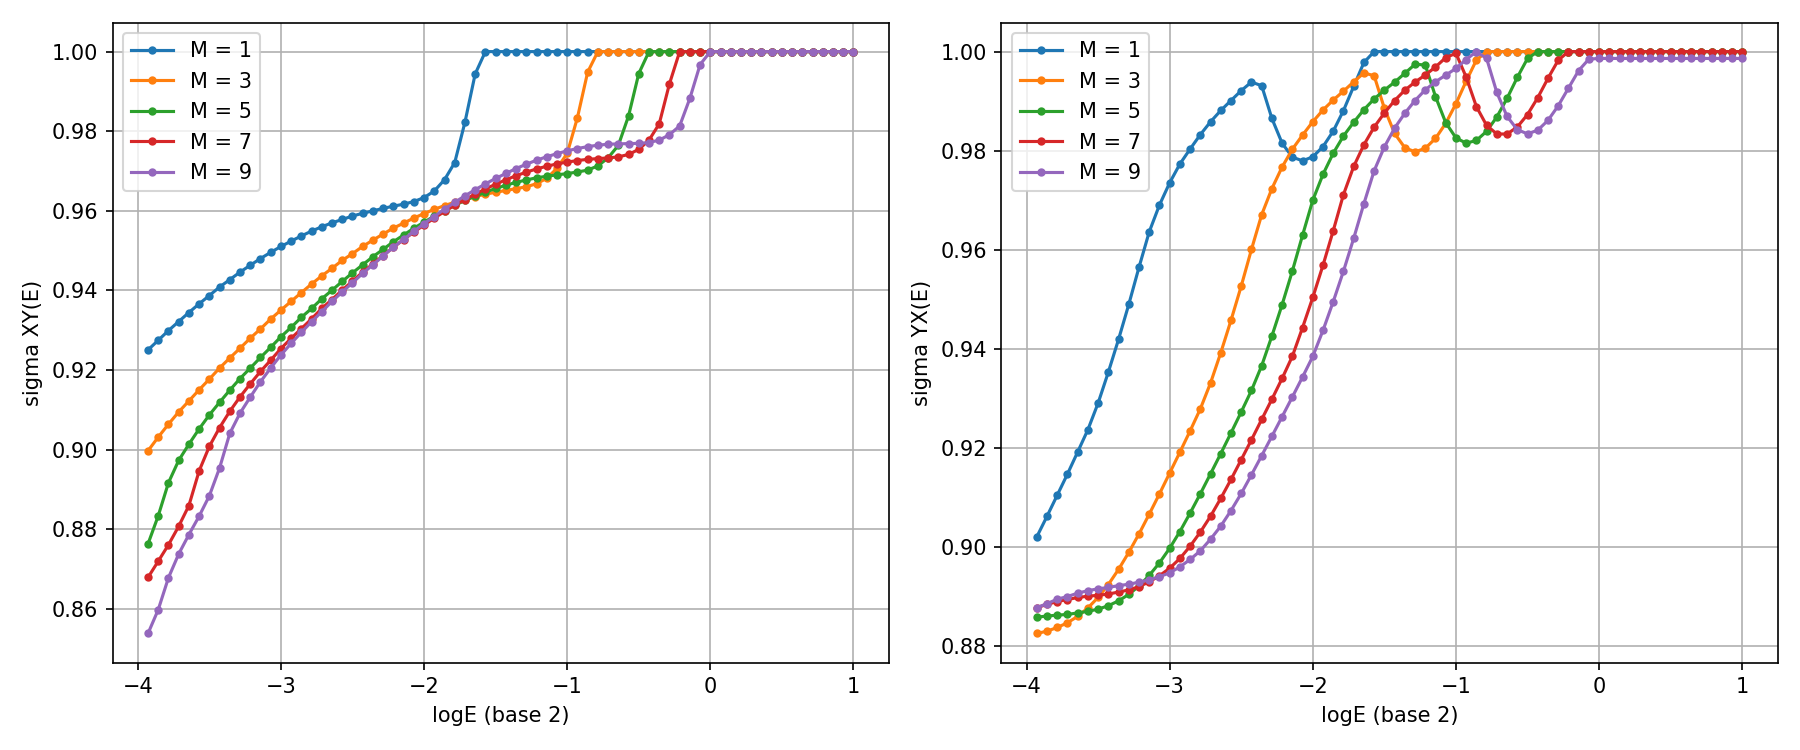
\includegraphics[scale=0.3]{vdp_test_figure_ding.png}\hspace{1em}
  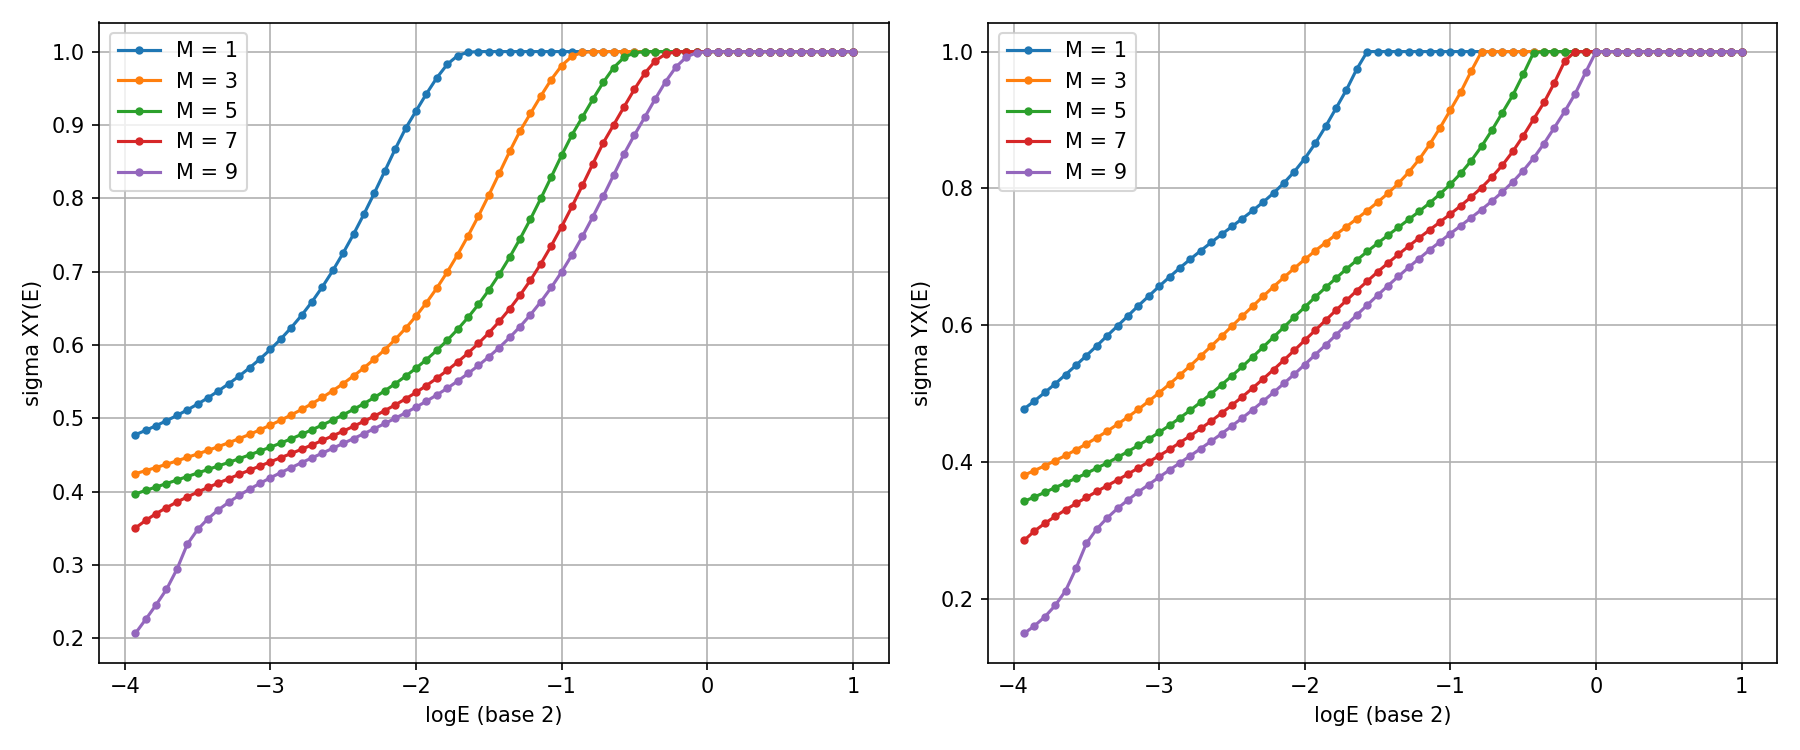
\includegraphics[scale=0.3]{vdp_test_figure_vm.png}
  \caption{
    Conditional dispersion curves for the synthetic Van der Pol tests.
    Left: strongly nonlinear “Ding’’ parameters, with modest separation of
    $\sigma_{XY}$ and $\sigma_{YX}$ and the largest relative asymmetry
    $|S_{XY}|$.  Right: near–limit–cycle “VM’’ parameters, where both
    directions exhibit very high nonlinear correlation but only a mild
    directional asymmetry.
  }
  \label{fig:vdp_sigma_combined}
\end{figure}



\printbibliography
\end{document}
